%!TEX program = xelatex
%!TEX encoding = UTF-8 Unicode
\documentclass[a5paper, twoside, 11pt]{article}

\usepackage{enumitem, amsmath, amssymb, tikz, fancyhdr, stackengine, sectsty, pdfpages}
\usepackage{lscape,longtable,amsmath,tabularx}
\usepackage{graphicx}

% размеры страницы
\usepackage[top=18mm, inner=10mm, outer=9mm, bottom=17mm, headheight=14.5pt, headsep=3mm, footskip=7mm]{geometry}

% пакет многоязыковой вёрстки
\usepackage[english, russian]{babel}

% настройки шрифтов
\usepackage{fontspec}

% свойства шрифтов по умолчанию
\defaultfontfeatures[\rmfamily, \sffamily]{Ligatures={TeX}}

% основной шрифт документа
\setmainfont{PTSerif-Regular}[
  Path=fonts/, Ligatures={TeX}, Scale=0.9,
  BoldFont={PTSerif-Bold},
  BoldItalicFont={PTSerif-BoldItalic},
  ItalicFont={PTSerif-Italic},
]

% шрифт без засечек
\setsansfont{PTSans-Regular}[
  Path=fonts/, Ligatures={TeX}, Scale=0.9,
  BoldFont={PTSans-Bold},
  BoldItalicFont={PTSans-BoldItalic},
  ItalicFont={PTSans-Italic},
]

% моноширинный шрифт
\setmonofont{consola}[Path=fonts/]

% шрифт для формул
\usepackage{unicode-math}
\setmathfont{latinmodern-math.otf}
\setmathfont{PTF56F}[Path=fonts/,range=\mathit/{latin,Latin}]
\setmathfont{PTF55F}[Path=fonts/,range=up]
\setmathfont{PTF55F}[Path=fonts/,range="2264-"2265]
\setmathfont{PTF55F}[Path=fonts/,range="003C-"003E]
% \setmathfont[range=\mathit/{greek,Greek}]{Arno Pro}

\allsectionsfont{\sffamily}

\usetikzlibrary{arrows.meta}

\usepackage{verbatim}
\usepackage{import}

\setlist[enumerate,1]{nolistsep}
\setlist[itemize,1]{nolistsep}

% русские названия заголовков разделов 
\newcommand{\problemsname}{Задачи}
\newcommand{\solutionsname}{Решения}
\newcommand{\inputname}{Формат входных данных}
\newcommand{\outputname}{Формат выходных данных}
\newcommand{\examplename}{Пример входного и выходного файлов}
\newcommand{\examplesname}{Примеры входного и выходного файлов}
\newcommand{\commentsname}{Комментарии}
\newcommand{\evaluationname}{Описание системы оценивания}
\newcommand{\InputFileName}{input.txt}
\newcommand{\OutputFileName}{output.txt}
\makeatletter
\def\kw@Explanation{Пояснение к примеру}
\def\kw@Explanations{Пояснения к примерам}

% заголовки разделов и~столбцов таблицы примеров
\newcommand{\problempartheading}[1]{\par\medskip\noindent\textbf{\sffamily #1}\par\penalty10000\noindent}
\newcommand{\InputFile}{\problempartheading{\inputname}}
\newcommand{\OutputFile}{\problempartheading{\outputname}}
\newcommand{\Comments}{\problempartheading{\commentsname}}
\newcommand{\Scoring}{\problempartheading{\evaluationname}}
\newcommand{\Example}{\par\medskip\noindent\textbf{\sffamily\examplename}\raisebox{-2pt}{\strut}\par\penalty10000\noindent}
\newcommand{\Examples}{\par\medskip\noindent\textbf{\sffamily\examplesname}\raisebox{-2pt}{\strut}\par\penalty10000\noindent}
\newcommand{\Note}{\Comments}
\newcommand{\Explanation}{\problempartheading{\kw@Explanation}}
\newcommand{\Explanations}{\problempartheading{\kw@Explanations}}

% русские знаки нестрогих неравенств
\renewcommand{\geq}{\geqslant}
\renewcommand{\leq}{\leqslant}
\renewcommand{\ge}{\geq}
\renewcommand{\le}{\leq}

% штрафы за разрыв строки по оператору
\binoppenalty=10000
\relpenalty=10000

\makeatletter
% задача = \begin{problem}{name}{in}{out}{TL}{ML}
\newenvironment{problem}[5]{%
  \subsection{#1}%
  \renewcommand{\InputFileName}{#2}%
  \renewcommand{\OutputFileName}{#3}%
}{}
\newenvironment{tutorial}[1]{\subsection{#1}}{}
\renewcommand{\thesubsection}{\Alph{subsection}.}
\renewcommand{\thesection}{}

% ширина таблицы примеров - по умолчанию равна ширине текста минус 2 красных строки
\newlength{\ex@mpwidth}
\setlength{\ex@mpwidth}{\textwidth}
\advance\ex@mpwidth-2\parindent
\advance\ex@mpwidth-4\tabcolsep

% ширины колонок ввода, вывода и~примеров для таблиц примеров
\newlength{\ex@mpinpwidth}
\newlength{\ex@mpoutwidth}
\newlength{\ex@mpcomwidth}

% -- Setup sizes --
\newlength{\thelinewidth}
\thelinewidth=\textwidth
\newlength{\exmpwidinf}
\newlength{\exmpwidouf}
\newlength{\exmpwidewid}
\newlength{\exmpthreewidinf}
\newlength{\exmpthreewidouf}
\newlength{\exmpthreewidnote}

\newif\ifintentionallyblankpages

\exmpwidinf=0.43\thelinewidth
\exmpwidouf=0.43\thelinewidth
\exmpwidewid=0.9\thelinewidth
\exmpthreewidinf=0.28\thelinewidth
\exmpthreewidouf=0.28\thelinewidth
\exmpthreewidnote=0.30\thelinewidth

% во всех примерах нужно следить за разрывами строк, вставлять знак комментария после завершения команды \exmp во избежание ненужных разрывов
% например \exmp{2 4}{3 5}%

% таблица примеров с 2 колонками (ввод и~вывод)
% :FIXME:

% This is magic, which delete space after verbatiminput
\addto@hook{\every@verbatim}{\topsep=0pt\relax}

\def\s@tm@cr@s{
  \def\widthin##1{\exmpwidinf=##1\relax}
  \def\widthout##1{\exmpwidouf=##1\relax}
  \def\stretchin##1{\advance\exmpwidinf by ##1\relax}
  \def\stretchout##1{\advance\exmpwidouf by ##1\relax}
  \@ifstar{
      \error Star must not be used in example environment any more
  }
}

\newenvironment{example}[1][]{
  \s@tm@cr@s#1
  \ttfamily\obeylines\obeyspaces\frenchspacing
  \newcommand{\exmp}[2]{
      \begin{minipage}[t]{\exmpwidinf}\rightskip=0pt plus 1fill\relax##1\medskip\end{minipage}&
      \begin{minipage}[t]{\exmpwidouf}\rightskip=0pt plus 1fill\relax##2\medskip\end{minipage}\\
      \hline
  }

  \newcommand{\exmpfile}[2]{
    \exmp{
        \verbatiminput{##1}
    }{
        \verbatiminput{##2}
    }%
  }


  \begin{tabular}{|l|l|}
      \hline
      \multicolumn{1}{|c|}{\bf\texttt{\InputFileName}}&
      \multicolumn{1}{|c|}{\bf\texttt{\OutputFileName}}\\
      \hline
}{
  \end{tabular}
}

% таблица примеров с 3 колонками (ввод, вывод, комментарий), три аргумента - доли колонок 
\newenvironment{examplecommented}[3]{
\setlength{\ex@mpinpwidth}{#1\ex@mpwidth}
\setlength{\ex@mpoutwidth}{#2\ex@mpwidth}
\setlength{\ex@mpcomwidth}{#3\ex@mpwidth}
\newcommand{\exmp}[3]{\begin{minipage}[t]{\ex@mpinpwidth}\raggedright\ttfamily ##1\medskip\end{minipage} &
                      \begin{minipage}[t]{\ex@mpoutwidth}\raggedright\ttfamily ##2\medskip\end{minipage} &
                      \begin{minipage}[t]{\ex@mpcomwidth} ##3\medskip\end{minipage}\\\hline%
}
\obeylines\obeyspaces\frenchspacing

\noindent\begin{tabular}{|l|l|l|}
\hline\multicolumn{1}{|c|}{\bf\texttt{\InputFileName}}&\multicolumn{1}{c|}{\bf\texttt{\OutputFileName}}&
\multicolumn{1}{c|}{\bf\texttt{\commentsname}}\\
\hline
}{\end{tabular}\smallskip}

% таблица примеров в~1 колонку. Один пример верстается в~4 строки (считая заголовки) на всю ширину таблицы
\newenvironment{examplewide}{
\advance\ex@mpwidth2\tabcolsep 
\ttfamily\obeylines\obeyspaces\frenchspacing
\newcommand{\exmp}[2]{
  \begin{tabular}{|c|}
  \hline
  \multicolumn{1}{|c|}{\bf\texttt{\InputFileName}}\\
  \hline
  \begin{minipage}[t]{\ex@mpwidth}\rightskip=0pt plus 1fill\relax\raggedright ##1 \medskip\end{minipage}\\
  \hline
  \multicolumn{1}{|c|}{\bf\texttt{\OutputFileName}}\\
  \hline
  \begin{minipage}[t]{\ex@mpwidth}\rightskip=0pt plus 1fill\relax\raggedright ##2 \medskip\end{minipage}\\%
  \hline
  \end{tabular}\smallskip
}
}{}

\makeatother

% колонтитулы
\pagestyle{fancy}
\makeatletter
\fancyhead[LE]{\small \@title }
\makeatother
\fancyhead[RE]{}
\fancyhead[LO]{2024--2025 учебный год}
\fancyhead[RO]{}

\newcommand\olympiad{*** ОПРЕДЕЛИТЕ ОЛИМПИАДУ КОМАНДОЙ \textbackslash olympiad !!! ***}

\AtBeginDocument{\sloppy}
\newcommand*{\hm}[1]{
  #1\nobreak\discretionary{}%
  {\hbox{$\mathsurround=0pt #1$}}{}
}

% Предисловие
\newcommand{\foreword}{
\noindent\centerline{\parbox{0.9\textwidth}{\centering\sloppy\textbf{\olympiad}}}

\medskip
\noindent\centerline{\textbf{Дорогие участники!}}
\medskip

Проверка ваших решений производится \emph{автоматически} на наборе тестов, учитывающем различные варианты исходных данных, чтобы система могла выставить наиболее объективную оценку.

Для каждого теста выполняется следующая процедура:
\smallskip
\begin{itemize}[nolistsep]
\item
Система создает входной файл с исходными данными теста.
\item 
Запускается ваша программа, которая должна прочитать этот файл и~записать ответ в выходной файл.
\item
Затем система проверяет созданный вашей программой файл и~выносит решение о его правильности. 
\end{itemize}

Именно поэтому ваша программа должна читать данные из файла, а не с клавиатуры, и вывод записывать тоже в файл. Ни в коем случае нельзя использовать ввод с клавиатуры (например, функцию \texttt{readkey} в Паскале), так как в этом случае ваша программа будет ждать ввода бесконечно (и будет снята с тестирования после превышения лимита времени). Также важно строго соблюдать формат выходного файла. 

Приведем простой способ чтения из файла и записи в файл на языке Паскаль:\\
\framebox{\parbox{\textwidth}{
\small\tt
\{ {\rm\textit{ в начале программы }}\/ \}\\
assign(input, 'taskname.in');  reset(input);\\
assign(output, 'taskname.out'); rewrite(output);\\
\{ {\rm\textit{ теперь обычные процедуры read, readln, write, writeln будут работать \\ с файлами, а не с клавиатурой / экраном}} \}\\
  …\\
\{ {\rm\textit{ в конце программы }}\/ \}\\
close(output);
}}

\bigskip
\noindent
Ко всем задачам предъявляются следующие технические требования:

\noindent\addstackgap[8pt]{
\begin{tabular}{@{}ll}
Имена входного и выходного файлов & \textbf{см. в примерах к~задаче}\\
Максимальное время работы на одном тесте & 1 секунда\\
Максимальный объем используемой памяти	& 256 мегабайт \\
\end{tabular}
}

\begin{center}
\textbf{Желаем удачи!}
\end{center}
}

\renewcommand{\olympiad}{XXII Республиканская командная олимпиада школьников \mbox{по программированию}}

% Колонтитулы
\fancyhead[LE]{XXII Республиканская командная олимпиада школьников}
\fancyhead[RE]{}
\fancyhead[RO]{2024--2025 учебный год}
\fancyhead[LO]{}

\begin{document}
\pagestyle{empty}

\begin{flushright} \it
  Эффективная и слаженная \\
  командная работа --- залог успеха!
\end{flushright}
\vskip -15mm

\includegraphics[width=3cm,height=3cm]{figures/logo.pdf}
\\[3cm]
\begin{center}
\huge
XXII РЕСПУБЛИКАНСКАЯ\\КОМАНДНАЯ\\ОЛИМПИАДА ШКОЛЬНИКОВ\\
ПО~ПРОГРАММИРОВАНИЮ
\end{center}
\vfill
\centerline{Якутск}
\centerline{6 апреля 2025 г.}

\newpage
\noindent XXII Республиканская командная олимпиада школьников по программированию.~--- Якутск, 2025.
\\[5mm]
Сборник содержит условия задач XXII Республиканской командной олимпиады школьников по программированию и возможные варианты решений. Олимпиада проводилась 6 апреля 2025~г. на базе Института математики и информатики СВФУ им. М.К. Аммосова при участии Малой академии наук РС~(Я) в г.~Якутск. Участникам было предложено за пять часов решить двенадцать задач.
\vfill
\hfill © Авторский коллектив, 2025

\newpage
\noindent
\textbf{СПОНСОРЫ ОЛИМПИАДЫ}
\\[7mm]
\begin{tabular}{ @{} p{.44\textwidth} p{.5\textwidth} }
  \raisebox{-5ex}{
\includegraphics[width=.43\textwidth]{figures/axioma.pdf}}
  & 
  ГЕНЕРАЛЬНЫЙ СПОНСОР\newline
  ООО «Аксиома»\newline
  \textit{директор \newline 
  Наталья Леонтьевна Махонина}
  \newline\strut
\\
  \raisebox{-4.7ex}{
\includegraphics{figures/cts.png}}
  & 
  ГК <<КопирТехСервис>>\newline
  \textit{Генеральный директор \newline
  Александр Тарасович Никифоров}
  \newline\strut
% \\
\end{tabular}

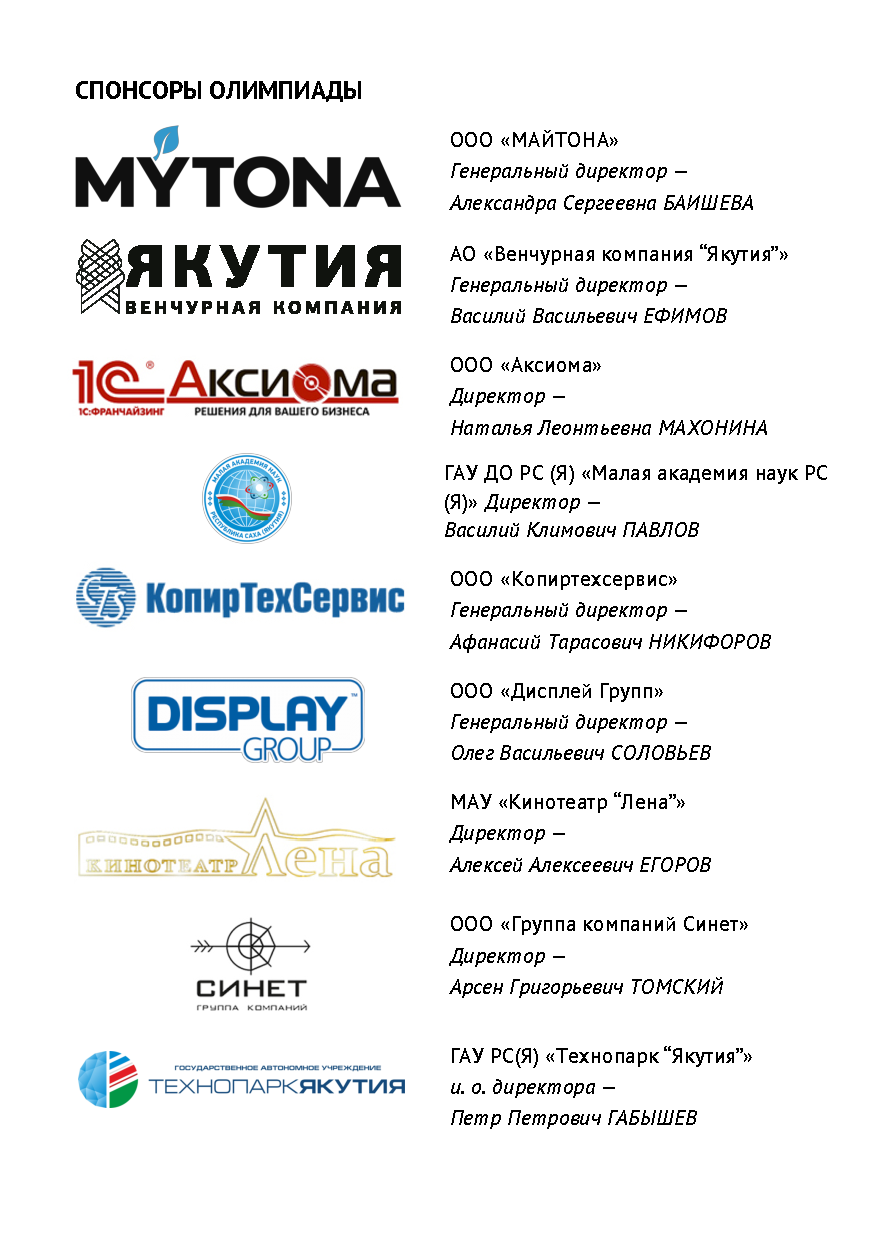
\includepdf{figures/logopage.pdf}

\newpage
\noindent
\textbf{ОРГКОМИТЕТ ОЛИМПИАДЫ}
% \\[2mm]
% ФЕДОРОВ Михаил Прокопьевич\\ 
% \textit{проректор по педагогическому образованию \\ 
% ФГАОУ ВО <<Северо-Восточный федеральный университет \\
% \textit{имени М.\,К. Аммосова>>~--- председатель}}
% \\[2mm]
% ПАВЛОВ Василий Климович  \\
% \textit{ректор Малой академии наук РС\,(Я)~--- 
% заместитель председателя}
% \\[2mm]
% ЛИ-ЦАЙ Мария Владимировна  \\
% \textit{главный специалист Министерства образования и науки РС~(Я)}
% \\[2mm]
% НИКОЛАЕВА Наталья Васильевна \\
% \textit
% {зав. кафедрой теории и методики обучения информатике ИМИ СВФУ, \\
% зав. кафедрой информатики Малой академии наук РС\,(Я)}
% \\[2mm]
% БУДИКИНА Людмила Евсеевна \\
% \textit
% {начальник учебного отдела Малой академии наук РС\,(Я)} 
% \\[2mm]
% КОРЯКИНА Туйара Васильевна \\
% \textit{методист кафедры информатики Малой академии наук РС\,(Я)}
% \\[2mm]

\newpage

\noindent
\textbf{ЖЮРИ ОЛИМПИАДЫ}
% \\[2mm]
% ПАВЛОВ Никифор Никитич \\
% \textit{к. ф.-м. н., доцент кафедры информационных технологий\\
% ИМИ СВФУ -- председатель}
% \\[2mm]
% ПАВЛОВ Александр Викторович \\
% \textit{к. ф.-м. н., доцент кафедры ИТ ИМИ СВФУ}
% \\[2mm]
% ПРОТОДЬЯКОНОВА Татьяна Гаврильевна \\
% \textit{к. ф.-м. н., учитель математики и информатики\\ Республиканского лицея-интерната}
% \\[2mm]
% ЛЕВЕРЬЕВ Владимир Семенович \\
% \textit{старший преподаватель кафедры ИТ ИМИ СВФУ}
% \\[2mm]
% СИТНИКОВ Сергей Иванович \\
% \textit{старший преподаватель кафедры теории и \\методики обучения информатике ИМИ СВФУ }
% \\[2mm]
% ЭВЕРСТОВ Владимир Васильевич \\
% \textit{старший преподаватель кафедры ИТ ИМИ СВФУ}
% \\[2mm]
% ДЬЯКОНОВ Айтал Викторович \\
% \textit{учитель информатики СУНЦ СВФУ - Университетского лицея и РЛИ,\\
% победитель международных олимпиад по информатике и математике}
% \\[2mm]
% НИКОЛАЕВА Наталья Васильевна \\
% \textit{к. ф.-м. н., зав. кафедрой ТМОИ ИМИ СВФУ,\\
% зав. кафедрой информатики МАН РС(Я) – секретарь}


\newpage
\newpage
\noindent
\textbf{СПИСОК УЧАСТНИКОВ}
\begin{description}

\item[11 Тестировщики Java] \textit{(11 кл. ЯГЛ, руководитель Жиркова М.\,М.)} \\
Афанасьев Федор Алексеевич, Иванов Дмитрий Максимович, \\
Исаев Андрей Васильевич

\item[BUG] \textit{(Бердигестяхская улусная гимназия им.\,В.\,В.\,Филиппова, рук. Сидорова Ф.\,Л.)} \\
Антонов Александр Дьулустанович \textit{9 кл.}, \\
Михайлов Айсен Михайлович \textit{11 кл.}, Старостин Василий Юрьевич \textit{11 кл.}

\item[Csmteam] \textit{(11 кл., Хатасская СОШ им.\,П.\,Н. и Н.\,Е.\,Самсоновых, рук. Петров П.\,П.)} \\
Абрамов Артем Александрович, Горохов Айсен Викторович, \\
Попов Максим Андреевич

\item[Ctrl+Alt+Elite] \textit{(ИТЛ №24 г.\,Нерюнгри им.\,Е.\,А.\,Варшавского, рук. Богданов Р.\,А.)} \\
Гурьев Артур Альбертович \textit{11 кл.}, Неграшев Денис Романович \textit{9 кл.}, \\
Неживых Дмитрий Андреевич \textit{11 кл.}

\item[enaije'es] \textit{(11 кл. РЛИ, руководитель Уваровская М.\,И.))} \\
Федоров Альберт Викторович, Каратаев Святослав Семенович, \\
Попов Кирилл Николаевич

\item[Eternity Gaming] \textit{(10 кл. Октемский НОЦ им.\,М.\,Е.\,Николаева, рук. Ковров Ф.\,Ф.)} \\
Афанасьев Леонид Владиславович, Никитин Егор Юрьевич, \\
Павлов Артём Дмитриевич

\item[eng54] \textit{(10 кл. РЛИ, руководитель Уваровская М.\,И.)} \\
Дормидонтов Ярослав Владимирович, Припузов Сулустаан Денисович, \\
Романов Альберт Сергеевич

\item[Junior] \textit{(9 кл. ЯГЛ, руководитель Жиркова М.\,М.)} \\
Жирков Ярослав Константинович, Мункуев Эрдэм Амирзаяаевич, \\
Попов Эльдар Леонидович

\item[КааКii] \textit{(11 кл. РЛИ, руководитель Уваровская М.\,И.)} \\
Колодезников Андрей Аркадьевич, Коркин Иннокентий Иосифович, \\
Ксенофонтов Артём Александрович

\item[MVP] \textit{(11 кл. Октемский НОЦ им.\,М.\,Е.\,Николаева, руководитель Ковров Ф.\,Ф.)} \\
Карпов Максим Григорьевич, Кузьмин Байдам Андреевич, \\
Федоров Кирилл Владимирович

\item[АТА-56] \textit{(8 кл. РЛИ, руководитель Николаева Н.\,В.)} \\
Илларионов Анатолий Анатольевич, Саввинов Айаан Юрьевич, \\
Чупров Артём Сергеевич

\item[Бо Сины] \textit{(СПЛ, руководители Саввинов И.\,С. и Фролова С.\,М.)} \\
Корякин Андрей Леонидович \textit{9 кл.}, Лаптев Данияр Антонович \textit{8 кл.}, \\
Припузов Дархан Денисович \textit{8 кл.}

\item[Дети Макарова] \textit{(Чурапчинская гимназия им.\,С.\,К.\,Макарова, рук. Захаров П.\,П.)} \\
Дьяконов Алексей Александрович \textit{7 кл.}, Петров Виктор Кузьмич \textit{8 кл.}, \\
Сивцев Аман Прокопьевич \textit{7 кл.}

\item[ЗФЯ] \textit{(СПЛ, руководители Саввинов И.\,С. и Фролова С.\,М.)} \\
Арьянов Янис Алексеевич \textit{11 кл.}, Захаров Нюргун Семенович \textit{10 кл.}, \\
Фёдоров Артём Афанасьевич \textit{11 кл.}

\item[КыыStar] \textit{(10 кл. РЛИ, руководитель Уваровская М.\,И.)} \\
Афанасьева Надежда Юрьевна, Винокурова Светлана Алексеевна, \\
Канаева Рената Артемовна

\item[Название команды] \textit{(11 кл. РЛИ, руководитель Уваровская М.\,И.)} \\
Малышев Виктор Валерьевич, Неустроева Нарыйаана Иннокентьевна, \\
Решетников Ньургун Петрович

\item[Саайса] \textit{(8 кл. Томпонская многопрофильная гимназия им.\,В.\,А.\,Штырова, \\
руководитель Рогачева Е.\,Г.)} \\
Илларионов Саян Васильевич, Новгородов Айсен Петрович, \\
Роев Айтал Нюргунович

\item[Сигмы] \textit{(9 кл. Айыы Кыһата, руководители Халабышева Е.\,В. и Готовцева Е.\,Д.)} \\
Семенова Майя Ньургуновна, Слободчиков Петр Павлович, \\
Тарский Иван Евгеньевич

\item[СУНЦ-1] \textit{(10 кл. СУНЦ СВФУ, руководитель Фролова С.\,М.)} \\
Евстифеев Игорь, Трофимова Диана, Халланова Айна

\item[СУНЦ-2] \textit{(10 кл. СУНЦ СВФУ, руководитель Фролова С.\,М.)} \\
Голиков Александр Алексеевич, \\
Абрамов Айдамир, \textit{10 класс} \\
Козьмин Виталий, \textit{10 класс}

\item[Фломастеры] \textit{(8 кл. СПЛ, рук. Саввинов И.\,С. и Фролова С.\,М.)} \\
Егоров Иван Иванович, Козлов Ньургун Степанович, \\
Назаров Руслан Ильич

\item[ФСБ] \textit{(8 кл. РЛИ, руководитель Николаева Н.\,В.)} \\
Большакова Амелия Егоровна, Слепцова Карина Гаврииловна, \\
Федорова Виктория Владиславовна

\item[ФТЛ-7] \textit{(7 кл. ФТЛ, руководитель Романов Ю.\,Н.)} \\
Местников Тимур, Григорьев Эрчим, Захаров Вячеслав

\item[ФТЛ-8] \textit{(8 кл. ФТЛ, рук. Куличкин Н.\,Н.)} \\
Васильева Ника Сарыаловна, Елизаров Василий Павлович, \\
Платонов Егор

\item[Ханалас 1] \textit{руководитель Егоров В.\,Д.} \\
Беца Максим Алексеевич \textit{8 кл. Покровская СОШ №3-ОЦ с УИОП}, \\
Марков Артур Гаврильевич \textit{9 кл. Покровская СОШ №1 им.\,И.\,М.\,Яковлева}, \\
Немечкин Артем Владимирович \textit{9 кл. Покровская СОШ №3-ОЦ с УИОП}

\item[Ханалас 2] \textit{(Покровская СОШ №2 с УИОП, руководитель Мордовской Д.\,А.)} \\
Боярский Дмитрий Владимирович \textit{8 кл.}, \\
Латышев Айгылаан Николаевич \textit{7 кл.}, \\
Федоров Алексей Васильевич \textit{9 кл.}

\item[ЧИН chinA] \textit{(10 кл. РЛИ, руководитель Уваровская М.\,И.)} \\
Иевлев Арылхан Маркович, Николаев Тимофей Дмитриевич, \\
Чашкин Георгий Фомич

\item[Чурапча] ~ \\
Александров Николай Васильевич \textit{10 кл. \\
(Чурапчинская СОШ им.\,С.\,А.\,Новгородова, руководитель Прокопьев~Е.\,В.)}, \\
Куличкина Кристина Федоровна \textit{10 кл.},
Павлов Артем Айаалович \textit{9 кл. (Чурапчинская гимназия им.\,С.\,К.\,Макарова, руководитель Захаров П.\,П.)}

\item[Эрэл54] \textit{(10 кл. РЛИ, руководитель Уваровская М.\,И.)} \\
Артемьев Георгий Иванович, Лыткин Марк Сергеевич, \\
Юмшанов Эрчим Петрович

\item[Эрэл55] \textit{(9 кл. РЛИ, руководитель Уваровская М.\,И.)} \\
Потапов Долан Васильевич, Сивцев Арсентий Андреевич, \\
Татаринов Тимур Иванович

\item[Эрэл57-1] \textit{(7 кл. РЛИ, руководитель Андреева Д.\,Д.)} \\
Колескин Артур Валерьевич, Уваровский Андрей Александрович, \\
Седалищев Михаил Петрович

\item[Эрэл57-2] \textit{(7 кл. РЛИ, руководитель Андреева Д.\,Д.)} \\
Васильев Бэргэн Егорович, Васильев Гансар Гаврильевич, \\
Васильев Дархан Валерьевич

\item[ЯГЛ] \textit{(10 кл. ЯГЛ, руководитель Жиркова М.\,М.)} \\
Лиханов Владимир Павлович, Серкин Алексей Александрович, \\
Христофоров Александр Дмитриевич

\item[ЯГНГ 10] \textit{(10 кл. ЯГНГ, руководители Спиридонов Я.\,Я. и Жерготов П.\,П.)} \\
Данилов Сандал Фёдорович, Евсеева Алина Владимировна, \\
Егоров Алексей Иванович

\item[ЯГНГ 11] \textit{(11 кл. ЯГНГ, рук. Спиридонов Я.\,Я. и Жерготов П.\,П.)} \\
Комиссаров Марат Юрьевич, Ксенофонтов Гектор Тимофеевич \\
Петухов Тимур Иннокентьевич

\end{description}

% \pagestyle{fancy}

% \newpage
% \rm
% \thispagestyle{plain}
% \section*{УСЛОВИЯ ЗАДАЧ}
% \addcontentsline{toc}{section}{Условия задач}
% \fancyhead[RO]{Условия задач}

% \newcommand{\importproblem}[1]{
%   \graphicspath{{problems/#1/statements/russian/}} %
%   \import{problems/#1/statements/russian/}{problem.tex} %
% }

% Контесты в Полигоне:
% [РКОШП-2025](https://polygon.codeforces.com/contest?contestId=49262)
% [РКЧПУ-2025](https://polygon.codeforces.com/contest?contestId=49263)
% [Все задачи](https://polygon.codeforces.com/contest?contestId=47811)

% \importproblem{thereandback}

%======================================================================
% \newpage
% \fancyhead[RO]{Решения}
% \section*{РЕШЕНИЯ}
% \addcontentsline{toc}{section}{Решения}
% \setcounter{subsection}{0}

% \renewcommand{\importproblem}[1]{
%   \graphicspath{{problems/#1/statements/russian/}} %
%   \import{problems/#1/statements/russian/}{tutorial.tex} %
% }

% \importproblem{thereandback}

% Результаты
% \begin{landscape}
% \input{results.tex}
% \end{landscape}

% \tableofcontents
\end{document}